\documentclass[12pt,a4paper]{article}
\usepackage[margin=1in]{geometry}
\usepackage{graphicx}
\usepackage{tikz}
\usetikzlibrary{shapes.geometric, arrows.meta, positioning, fit, backgrounds}
\usepackage{listings}
\usepackage{xcolor}
\usepackage{hyperref}
\usepackage{enumitem}
\usepackage{booktabs}
\usepackage{fancyhdr}
\usepackage{titlesec}

\hypersetup{colorlinks=true,linkcolor=blue,urlcolor=blue}
\pagestyle{fancy}
\fancyhf{}
\rhead{DevOps CI/CD Pipeline Project}
\lhead{IOE Project Report}
\cfoot{\thepage}

\lstset{
  basicstyle=\ttfamily\small,
  backgroundcolor=\color{gray!10},
  frame=single,
  breaklines=true,
  keywordstyle=\color{blue},
  commentstyle=\color{green!50!black},
  stringstyle=\color{red!70!black},
  showstringspaces=false
}

\titleformat{\section}{\Large\bfseries}{\thesection}{1em}{}
\titleformat{\subsection}{\large\bfseries}{\thesubsection}{1em}{}

\begin{document}

% ============================================================
% TITLE PAGE
% ============================================================
\begin{titlepage}
\centering
\vspace*{2cm}
{\Large\textbf{Institute of Engineering (IOE)}}\\[0.3cm]
{\large Tribhuvan University}\\[1.5cm]

{\Huge\textbf{Automated CI/CD Pipeline}}\\[0.3cm]
{\Huge\textbf{with Containerized Deployment}}\\[0.3cm]
{\Huge\textbf{and Monitoring}}\\[1.5cm]

{\Large\textit{Real Estate Buyer Portal --- A DevOps Project}}\\[2cm]

{\large
\textbf{Submitted by:}\\[0.3cm]
Ankit Belbase\\[1.5cm]

\textbf{Submitted to:}\\[0.3cm]
Department of Computer and Electronics Engineering\\[1.5cm]
}

{\large May 2026}
\end{titlepage}

% ============================================================
% 1. INTRODUCTION
% ============================================================
\section{Introduction}

\subsection{Background}
DevOps bridges the gap between software development and IT operations through automation, continuous integration, and continuous delivery. This project demonstrates a complete DevOps pipeline for a containerized web application, where code changes pushed to a Version Control System are automatically tested, built, deployed, and monitored --- with minimal manual intervention.

\subsection{Problem Statement}
Traditional software deployment involves manual steps: testing code locally, building artifacts, copying files to servers, and restarting services. This process is error-prone, slow, and inconsistent. The goal is to automate the entire workflow so that a single \texttt{git push} triggers testing, building, deployment, and health verification automatically.

\subsection{Objectives}
\begin{enumerate}
    \item Develop a full-stack web application containerized with Docker.
    \item Implement an automated 3-stage CI/CD pipeline using GitHub Actions.
    \item Set up real-time monitoring using Prometheus and Grafana.
    \item Provide infrastructure automation using Ansible and Terraform.
    \item Ensure changes are reflected in the running application once code is pushed to the VCS.
\end{enumerate}

\subsection{Scope}
The project covers the complete DevOps lifecycle: version control, automated testing, containerization, CI/CD pipelines, deployment automation, and infrastructure monitoring.

% ============================================================
% 2. SYSTEM ARCHITECTURE
% ============================================================
\section{System Architecture}

Figure~\ref{fig:architecture} shows the overall system architecture. When a developer pushes code to GitHub, the CI/CD pipeline triggers automatically. The pipeline runs three stages on the cloud, and upon completion, the application is deployed locally using Docker Compose. Prometheus scrapes metrics from the running application, and Grafana provides visualization dashboards.

\begin{figure}[h!]
\centering
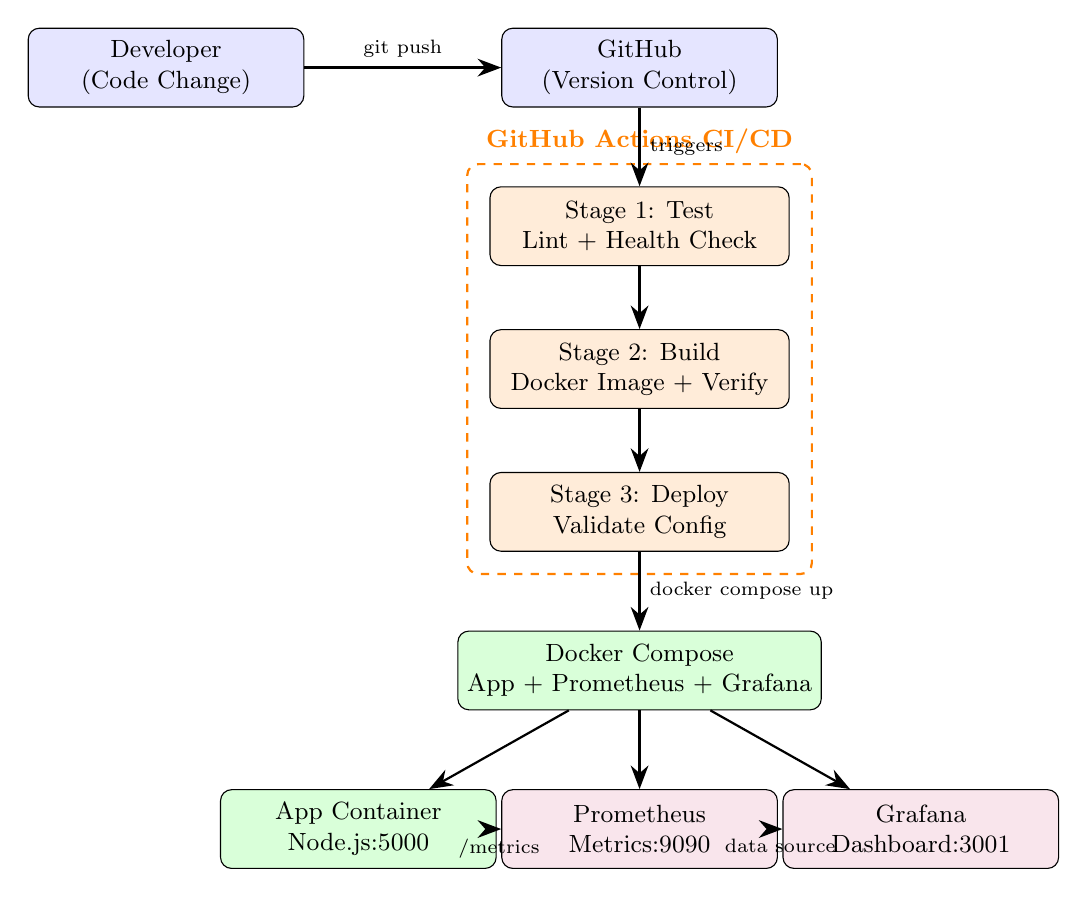
\begin{tikzpicture}[
    node distance=1.2cm and 2cm,
    box/.style={rectangle, draw, rounded corners, fill=blue!10, minimum width=3.5cm, minimum height=1cm, align=center, font=\small},
    cibox/.style={rectangle, draw, rounded corners, fill=orange!15, minimum width=3.8cm, minimum height=1cm, align=center, font=\small},
    deploybox/.style={rectangle, draw, rounded corners, fill=green!15, minimum width=3.5cm, minimum height=1cm, align=center, font=\small},
    monbox/.style={rectangle, draw, rounded corners, fill=purple!10, minimum width=3.5cm, minimum height=1cm, align=center, font=\small},
    arr/.style={-{Stealth[length=3mm]}, thick}
]
    % Nodes
    \node[box] (dev) {Developer\\(Code Change)};
    \node[box, right=2.5cm of dev] (vcs) {GitHub\\(Version Control)};
    
    \node[cibox, below=1cm of vcs] (test) {Stage 1: Test\\Lint + Health Check};
    \node[cibox, below=0.8cm of test] (build) {Stage 2: Build\\Docker Image + Verify};
    \node[cibox, below=0.8cm of build] (deploy) {Stage 3: Deploy\\Validate Config};
    
    \node[deploybox, below=1cm of deploy] (compose) {Docker Compose\\App + Prometheus + Grafana};
    
    \node[deploybox, below left=1cm and -0.5cm of compose] (app) {App Container\\Node.js:5000};
    \node[monbox, below=1cm of compose] (prom) {Prometheus\\Metrics:9090};
    \node[monbox, below right=1cm and -0.5cm of compose] (graf) {Grafana\\Dashboard:3001};
    
    % Arrows
    \draw[arr] (dev) -- node[above, font=\scriptsize] {git push} (vcs);
    \draw[arr] (vcs) -- node[right, font=\scriptsize] {triggers} (test);
    \draw[arr] (test) -- (build);
    \draw[arr] (build) -- (deploy);
    \draw[arr] (deploy) -- node[right, font=\scriptsize] {docker compose up} (compose);
    \draw[arr] (compose) -- (app);
    \draw[arr] (compose) -- (prom);
    \draw[arr] (compose) -- (graf);
    \draw[arr] (app) -- node[below, font=\scriptsize] {/metrics} (prom);
    \draw[arr] (prom) -- node[below, font=\scriptsize] {data source} (graf);
    
    % Grouping - CI/CD
    \begin{scope}[on background layer]
        \node[draw=orange, dashed, thick, rounded corners, fit=(test)(build)(deploy), inner sep=8pt, label={[font=\small\bfseries, orange]above:GitHub Actions CI/CD}] {};
    \end{scope}
    
\end{tikzpicture}
\caption{System Architecture Diagram}
\label{fig:architecture}
\end{figure}

% ============================================================
% 3. TECHNOLOGY STACK
% ============================================================
\section{Technology Stack}

\begin{table}[h!]
\centering
\begin{tabular}{@{}ll@{}}
\toprule
\textbf{Component} & \textbf{Technology} \\
\midrule
Web Application & Node.js, Express.js, SQLite, HTML/CSS/JS \\
Containerization & Docker, Docker Compose \\
CI/CD Pipeline & GitHub Actions (3-stage pipeline) \\
Monitoring & Prometheus + Grafana \\
Configuration Management & Ansible \\
Infrastructure as Code & Terraform (Docker provider) \\
Version Control & Git + GitHub \\
VM Provisioning & VirtualBox \\
\bottomrule
\end{tabular}
\caption{Technology Stack}
\end{table}

% ============================================================
% 4. IMPLEMENTATION
% ============================================================
\section{Implementation}

\subsection{Application Development}
The Buyer Portal is a full-stack web application built with Node.js and Express.js. It features user authentication (register/login with JWT), property browsing with filters, and a favourites system. The frontend uses vanilla HTML, CSS, and JavaScript with a modern glassmorphism design.

Key API endpoints:
\begin{itemize}[nosep]
    \item \texttt{POST /api/auth/register} --- User registration
    \item \texttt{POST /api/auth/login} --- User login (returns JWT)
    \item \texttt{GET /api/properties} --- List all properties
    \item \texttt{GET /api/favourites} --- User's saved properties
    \item \texttt{GET /api/health} --- Health check endpoint
    \item \texttt{GET /metrics} --- Prometheus metrics
\end{itemize}

\begin{center}
\fbox{\parbox{0.85\textwidth}{\centering\vspace{2cm}\textbf{PLACEHOLDER: Screenshot of the Buyer Portal Login Page}\\(http://localhost:5000)\vspace{2cm}}}
\end{center}

\begin{center}
\fbox{\parbox{0.85\textwidth}{\centering\vspace{2cm}\textbf{PLACEHOLDER: Screenshot of the Dashboard with Properties}\\(http://localhost:5000/dashboard.html)\vspace{2cm}}}
\end{center}

\subsection{Containerization with Docker}
The application is containerized using a Dockerfile based on \texttt{node:20-alpine}. Docker Compose orchestrates three services:

\begin{lstlisting}[language=bash, caption=Dockerfile]
FROM node:20-alpine
WORKDIR /app
COPY backend/package*.json ./backend/
WORKDIR /app/backend
RUN npm install --omit=dev
WORKDIR /app
COPY backend ./backend
COPY frontend ./frontend
EXPOSE 5000
CMD ["node", "backend/server.js"]
\end{lstlisting}

\textbf{Docker Compose Services:}
\begin{enumerate}[nosep]
    \item \textbf{app} --- Node.js application on port 5000 (with health check)
    \item \textbf{prometheus} --- Metrics scraper on port 9090
    \item \textbf{grafana} --- Visualization dashboard on port 3001
\end{enumerate}

\begin{center}
\fbox{\parbox{0.85\textwidth}{\centering\vspace{2cm}\textbf{PLACEHOLDER: Screenshot of \texttt{docker ps} showing 3 running containers}\vspace{2cm}}}
\end{center}

\subsection{CI/CD Pipeline with GitHub Actions}
The pipeline is defined in \texttt{.github/workflows/ci-cd.yml} and triggers on every push or pull request to the \texttt{main} branch.

\textbf{Stage 1 --- Lint \& Test:}
\begin{itemize}[nosep]
    \item Installs Node.js 20 and backend dependencies
    \item Runs syntax validation (\texttt{node -c server.js})
    \item Starts the server and verifies \texttt{/api/health} returns HTTP 200
    \item Verifies the \texttt{/metrics} endpoint is accessible
\end{itemize}

\textbf{Stage 2 --- Build Docker Image:}
\begin{itemize}[nosep]
    \item Builds Docker image tagged with commit SHA and \texttt{latest}
    \item Runs a test container from the built image
    \item Verifies health check inside the container
    \item Stops and removes the test container
\end{itemize}

\textbf{Stage 3 --- Deploy:}
\begin{itemize}[nosep]
    \item Only runs on pushes to \texttt{main} (not on PRs)
    \item Validates the \texttt{docker-compose.yml} configuration
    \item Deployment is performed locally using \texttt{docker compose up -d --build}
\end{itemize}

\begin{center}
\fbox{\parbox{0.85\textwidth}{\centering\vspace{2cm}\textbf{PLACEHOLDER: Screenshot of GitHub Actions showing all 3 stages passing (green checks)}\\(GitHub Actions page)\vspace{2cm}}}
\end{center}

\begin{center}
\fbox{\parbox{0.85\textwidth}{\centering\vspace{2cm}\textbf{PLACEHOLDER: Screenshot of Stage 1 (Test) logs showing health check passed}\vspace{2cm}}}
\end{center}

\subsection{Automated Local Deployment}
A deployment script (\texttt{scripts/push-and-deploy.ps1}) automates the full workflow in a single command:

\begin{lstlisting}[caption=Deployment Flow]
powershell -ExecutionPolicy Bypass -File scripts\push-and-deploy.ps1
\end{lstlisting}

This script performs four steps automatically:
\begin{enumerate}[nosep]
    \item Commits any uncommitted changes
    \item Pushes to GitHub (triggering CI pipeline)
    \item Rebuilds and redeploys Docker containers locally
    \item Runs a health check to confirm the app is live
\end{enumerate}

\begin{center}
\fbox{\parbox{0.85\textwidth}{\centering\vspace{2cm}\textbf{PLACEHOLDER: Screenshot of push-and-deploy.ps1 output showing all 4 steps passing}\vspace{2cm}}}
\end{center}

\subsection{Monitoring with Prometheus \& Grafana}

\textbf{Prometheus} scrapes the \texttt{/metrics} endpoint every 15 seconds. The application exposes custom metrics using \texttt{prom-client}:
\begin{itemize}[nosep]
    \item HTTP request duration histogram (by method, route, status code)
    \item Default Node.js metrics (CPU, memory, event loop, GC)
\end{itemize}

\textbf{Grafana} is auto-provisioned with:
\begin{itemize}[nosep]
    \item Pre-configured Prometheus datasource
    \item Pre-built dashboard with 6 panels showing app health
    \item No manual setup needed --- works out of the box
\end{itemize}

\begin{center}
\fbox{\parbox{0.85\textwidth}{\centering\vspace{2cm}\textbf{PLACEHOLDER: Screenshot of Prometheus query showing metrics}\\(http://localhost:9090)\vspace{2cm}}}
\end{center}

\begin{center}
\fbox{\parbox{0.85\textwidth}{\centering\vspace{2cm}\textbf{PLACEHOLDER: Screenshot of Grafana dashboard with monitoring panels}\\(http://localhost:3001)\vspace{2cm}}}
\end{center}

\subsection{Infrastructure Automation}

\textbf{Ansible Playbook} (\texttt{ansible/deploy.yml}) automates deployment to remote servers:
\begin{itemize}[nosep]
    \item Installs Docker on the target machine
    \item Clones the repository
    \item Builds and starts containers via Docker Compose
    \item Verifies deployment health
\end{itemize}

\textbf{Terraform Configuration} (\texttt{terraform/main.tf}) provisions Docker infrastructure as code:
\begin{itemize}[nosep]
    \item Creates a Docker network
    \item Provisions all 3 containers with proper port mappings
    \item Manages infrastructure state
\end{itemize}

% ============================================================
% 5. RESULTS AND TESTING
% ============================================================
\section{Results and Testing}

\subsection{CI/CD Pipeline Results}
The pipeline was tested with multiple code pushes. Each push triggered the full 3-stage pipeline:

\begin{table}[h!]
\centering
\begin{tabular}{@{}llll@{}}
\toprule
\textbf{Stage} & \textbf{Duration} & \textbf{Status} & \textbf{Checks Performed} \\
\midrule
Lint \& Test & ~30s & Pass & Syntax, health, metrics \\
Build Image & ~60s & Pass & Image build, container test \\
Deploy & ~15s & Pass & Config validation \\
\bottomrule
\end{tabular}
\caption{Pipeline Stage Results}
\end{table}

\subsection{Deployment Verification}
After running the push-and-deploy script, the following was verified:

\begin{itemize}[nosep]
    \item Health endpoint returns \texttt{\{"status":"ok"\}} with HTTP 200
    \item All 3 Docker containers are running and healthy
    \item Prometheus is scraping metrics successfully
    \item Grafana dashboard panels show live data
    \item Code changes (e.g., brand name change) are reflected immediately in the running app
\end{itemize}

\begin{center}
\fbox{\parbox{0.85\textwidth}{\centering\vspace{2cm}\textbf{PLACEHOLDER: Screenshot of /api/health endpoint showing updated response}\vspace{2cm}}}
\end{center}

\begin{center}
\fbox{\parbox{0.85\textwidth}{\centering\vspace{2cm}\textbf{PLACEHOLDER: Screenshot of the app showing the changed brand name after deployment}\vspace{2cm}}}
\end{center}

% ============================================================
% 6. CHALLENGES FACED
% ============================================================
\section{Challenges Faced}

\begin{enumerate}
    \item \textbf{Docker Build Caching:} Initial builds were slow (~3 min). By ordering Dockerfile layers correctly (copying \texttt{package.json} before source code), subsequent builds use cache and complete in seconds.
    
    \item \textbf{GitHub Actions Free Tier:} The free tier has limited minutes. The pipeline was optimized to run only essential checks, keeping total CI time under 2 minutes.
    
    \item \textbf{Prometheus Metrics Integration:} Integrating \texttt{prom-client} required careful histogram bucket configuration and label naming to produce useful metrics without high cardinality.
    
    \item \textbf{Grafana Auto-Provisioning:} Configuring Grafana to auto-load datasources and dashboards on startup required specific directory structures and YAML configuration files.
    
    \item \textbf{Cross-Platform Scripting:} Deployment scripts needed to work on both Windows (PowerShell) and Linux (Bash) environments, requiring careful handling of path separators and command syntax.
\end{enumerate}

% ============================================================
% 7. CONCLUSION
% ============================================================
\section{Conclusion}

This project successfully demonstrates a complete DevOps pipeline for a containerized web application. The key achievements are:

\begin{itemize}
    \item A fully functional Real Estate Buyer Portal containerized with Docker
    \item An automated 3-stage CI/CD pipeline using GitHub Actions that triggers on every code push
    \item Real-time application monitoring using Prometheus and Grafana with auto-provisioned dashboards
    \item Infrastructure automation using Ansible and Terraform
    \item A single-command deployment script that pushes code, triggers CI, deploys locally, and verifies health --- achieving the goal of changes being reflected in the running application once code is committed to the VCS
\end{itemize}

The project demonstrates that even with free-tier tools and local infrastructure, a production-grade DevOps workflow can be implemented, providing automated testing, containerized deployment, and comprehensive monitoring.

\end{document}
